\date{September 2020}

\documentclass[conference]{IEEEtran}
\usepackage{xcolor}
\usepackage[utf8]{inputenc}
\usepackage{graphicx}
\usepackage{fixltx2e}
\usepackage{upgreek}
\usepackage{amsmath}
\usepackage{amsfonts}
\usepackage{amssymb}
\usepackage{mathtools}
\usepackage{float}
\usepackage{multicol}
\usepackage{blkarray}
\usepackage{tabularx}
\usepackage{gensymb}
\usepackage{subcaption}
\usepackage[font=small,labelfont=bf]{caption}
\usepackage{pgfgantt} % Gantt chart package
\PassOptionsToPackage{hyphens}{url}\usepackage{hyperref} % line breaks for links with the \url command
\usepackage{rotating} % landscape figures
\usepackage{comment} % multiline comments
\usepackage{listings}

\lstset{
  aboveskip=3mm,
  belowskip=3mm,
  showstringspaces=false,
  columns=flexible,
  basicstyle={\small\ttfamily},
  numbers=none,
  breaklines=true,
  breakatwhitespace=true,
  tabsize=3
}

% \usepackage[style=ieee]{biblatex}
% \addbibresource{references.bib}

\title{Convolutional Autoencoders}

\author{\IEEEauthorblockN{David Pomerenke, JingYang Zeng} 
\textit{Advanced Concepts of Machine Learning (Kurt Driessens) 2020} \\
\IEEEauthorblockA{\textit{Department of Data Science and Knowledge Engineering, Maastricht University}
}} 


% comment possibilities for all authors
\usepackage{color}
\usepackage{xcolor}
\newcommand{\todo}[1]{\textcolor{violet}{TODO #1}} % dp is already defined

\begin{document}

\maketitle

\thispagestyle{plain} % page numbers!
\pagestyle{plain} % page numbers!

\begin{abstract}
    We use the Keras framework to create a more complex convolutional autoencoder model, and successfully apply it to image data. We explore the impact of different architectures. We try to apply our model to an image colorization problem.
\end{abstract}

% \tableofcontents


\section{Implementation}

We use Jupyter Notebbook to annotate our implementation, the code is accessible via the google colab\footnote{\url{https://colab.research.google.com/drive/1lN6BkHgbCY84mS2KZzOX-JUWm1n_UY8k?usp=sharing#scrollTo=gYXe0msFWz0w}}. 

We implement the autoencoder neural network in Python, making use of the \textit{Keras} library\footnote{\url{https://https://keras.io/}} as our neural network framework. 

we train an autoencoder with the parameters suggested in the assignment. At first, we load the training data from Keras directly\footnote{\url{https://www.cs.toronto.edu/~kriz/cifar.html}}. Then we divide the data into three data set for the train, test and validation.

% The encoder will be constructed by a stack of Conv2D and MaxPooling2D layers, meanwhile the decoder will consist in a stack of Conv2D and UpSampling2D layers. 
% We start encoding with the convolutional kernel at size 8, then apply a max pool with the size 2 * 2. 
% We additionally repeat the process above twice but set different size of kernel at size 16 and 32. 

%After getting the encoded result, we begin dealing with decoder process. We apply the UpSampling layer before decoding by convolution kernel, then apply the convolution kernel. Similarly, we repeat the stucture three time with difference convolution kernel size at 8, 16 and 32.


The sigmoid function $f(x) = \frac{1}{1+e^{-x}}$ is not recommended for the autoencoder algorithm as kernel but it is still works if we set a larger epoch amount. However, the rectifier $f(x) = \max(0,x)$, can achieve a better and quicker global optimization.

Autoencoders do not only provide a different way to reduce noise with traditional filter such as Sobel filters, they also can restrain the information during the process of compressing the image.

\section{Reconstruction}

For the first model (specified in the assignment), the evolution of the error can be seen in figure \ref{fig:bestandworst}. The test error is $0.57$ after 10 epochs. The latent space has a size of $\left(\frac{W-K+2P}{S}+1\right)^2\cdot C = \left(\frac{8-3+2\cdot 1}{1}+1\right)^2\cdot 16 = 1024$.


\begin{figure}
    \centering
    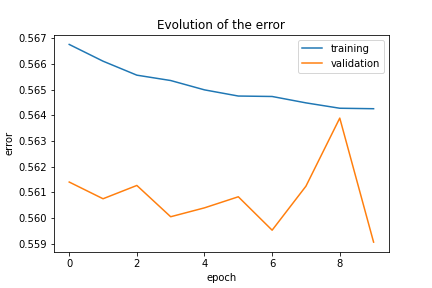
\includegraphics[width=8cm]{error_evolution_first_model.png}
    \caption{Accuracy given the learning rate and the number of iterations.}
    \label{fig:performance}
\end{figure}

We also test the impact of different architectures and hyperparameters. In order to evaluate multiple architectures, we adapt our model to allow for the specification of hyperparameters and parameters with regard to the architecture. We check all combinations of the following variable configurations:

\begin{enumerate}
    \item \textit{Fewer layers (binary):} If true, then the medium-sized convolutions between the first / last convolutions and the latent space are omitted; so there are only three rather than 5 convolutions.
    \item \textit{Channel factor (1, 2, 4):} We divide the number of channels for all convolutions by two and then apply a channel factor from the set (thus, halving, keeping, and doubling the number of channels). 
    \item \textit{Kernel size (3, 5):} We vary the kernel size between 3 and 5. We combine this with a variation of the padding (see the implementation of the \textit{conv} function), such that the kernel size does not influence the output size of the convolution.
    \item \textit{Compression factor (1, 2, 4):} A factor for the max pooling and upsampling layers, where $2$ corresponds to the compression of the first model. 
\end{enumerate}

This results in $2\cdot3\cdot2\cdot3=36$ different models. The correlation of the size of the latent space and the reconstruction error within these models is displayed in Figure \ref{fig:re}. After sorting by accuracy, we can get the best model and worst model, see Figure \ref{fig:bestandworst}.

\begin{figure}
    \centering
    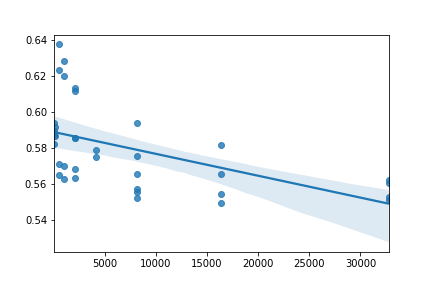
\includegraphics[width=8cm]{reconstruction_error_vs_latent_space_size.png}
    \caption{Reconstruction error given the latent space size.}
    \label{fig:re}
\end{figure}

\begin{figure}
    \centering
    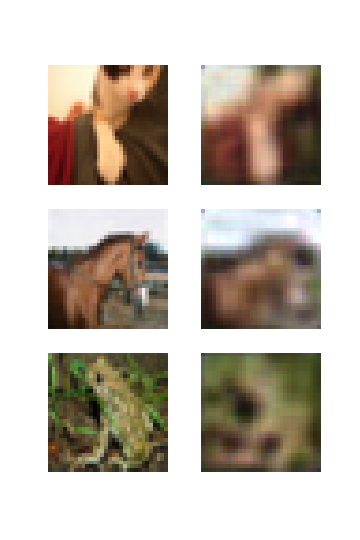
\includegraphics[width=2.5cm]{first.png}
    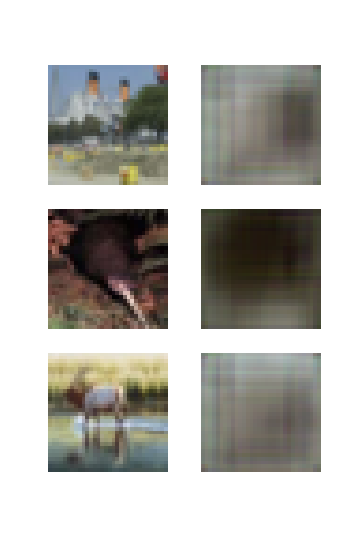
\includegraphics[width=2.5cm]{worst.png}
    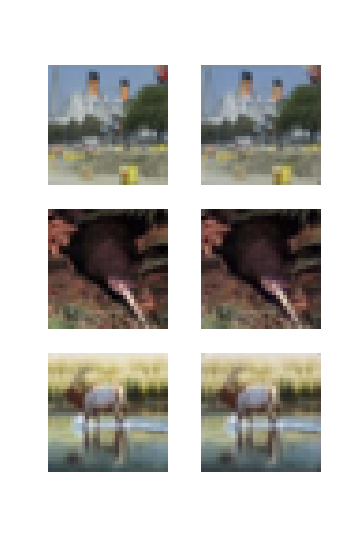
\includegraphics[width=2.5cm]{best_10.png}
    \caption{Original (left each) and predictions (right each) for the first configuration (as given in the assignment, left), worst configuration (center), and best configuration (right) with 10 training epochs on 10\% of the data. }
    \label{fig:bestandworst}
\end{figure}

\newpage

\section{Colorization}

We try three different approaches to encoding the colour information of images separately from their grayscale values: 

\begin{enumerate}
    \item We implement conversion to and from the $YC_bC_r$ colour space. This should be the optimal way of separating the colour information, and it is widely used in video compression. While it works, it leads to unexpected results when we train our best previous CNN model (slightly adapted for the number of input and output dimensions) with grayscale ($Y$) input data and $C_bC_r$ output data: The predicted values seem to somehow correlate with the actual colours, but not in the correct way; see Figure~\ref{fig:g1}. We try to apply some constant linear transformations of the values in order to correct this, but without success. Therefore, we try out different approaches to encoding the colour information only. 
    \item We try to encode the colour information by \textit{dividing} each colour layer by the grayscale layer (now, unlike $Y$ above, the average of the three colour layers). We make some visualizations of this encoding and think that it does not capture the colour information well.
    \item We encode the colour information by \textit{subtracting} the grayscale layer from each colour layer, see Figure~\ref{fig:genc}. Test visualizations show that this yields a very intuitive encoding of the colour information. However, the predictions of the thus trained network are very poor, and the predicted colours do not even seem to correlate with the real in any way; see Figure~\ref{fig:g2}.
\end{enumerate}

\begin{figure}[b]
    \centering
    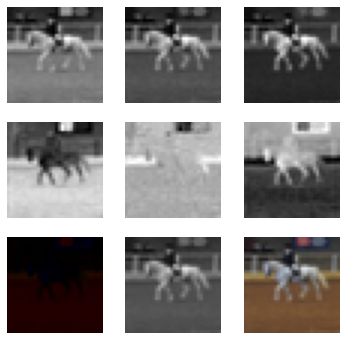
\includegraphics[width=4cm]{encoding.png}
    \caption{Representation of an image as RGB differences. In order from left to right: R, G, B values each; R, G, B differences from the grayscale each; grayscale; R, G, B differences combined; reconstructed colour image from R, G, B differences and grayscale.}
    \label{fig:genc}
\end{figure}

\begin{figure}[b]
    \centering
    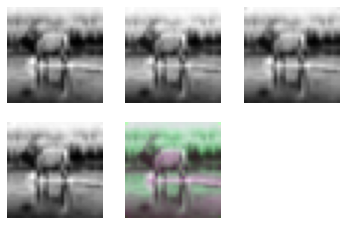
\includegraphics[width=4cm]{gray_1.png}
    \caption{Predicted colorization according to the first model (trained 100 epochs on 10\% of the data). In order from left to right: True $C_b$ chroma value, true $C_r$ chroma value, predicted $C_b$ chroma value, predicted $C_r$ chroma value, chroma combined with true $y$ value (= final colorization prediction). The colours are somewhat aligned to the objects, but they do not match the true colours.}
    \label{fig:g1}
\end{figure}

\begin{figure}[b]
    \centering
    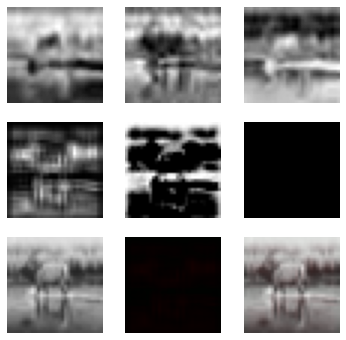
\includegraphics[width=4cm]{gray_2.png}
    \caption{Predicted colorization according to the second model (trained 100 epochs on 10\% of the data. In order from left to right: True R, G, B differences each; predicted R, G, B differences each; grayscale; combined R, G, B differences; combined grayscale and RGB values (=final colorization prediction). The predictions just cover all images in an overall tone of light brown.}
    \label{fig:g2}
\end{figure}

% \printbibliography

\newpage


\end{document}